%        File: learnability.tex
%     Created: Mon Feb 06 11:00 AM 2017 E
% Last Change: Mon Feb 06 11:00 AM 2017 E
%
% arara: pdflatex: {options: "-draftmode"}
% arara: biber
% arara: pdflatex: {options: "-draftmode"}
% arara: pdflatex: {options: "-file-line-error-style"}
\documentclass[MilwayThesis]{subfiles}

\begin{document}
In this section, I will evaluate some previous analyses of resultatives, based on their learnability, largely setting aside questions of over-/under-generation.
This choice of evaluation metric is motivated by the overall goals of this thesis and by the fact that questions of generative capacity are well-addressed by the analyses that I will evaluate.


One approach to the resultative parameter is what I will call the lexicalization account.
Under this account, event descriptions are decomposable into several universal features (\textit{e.g.}, \textsc{Result}, \textsc{Manner}, \textsc{Process}), and language variation results from languages lexicalizing these features differently.
One such an account by \textcite{son2008microparameters} proposes that English and German lexicalize \textsc{Result} in null heads, while Romance languages only lexicalize \textsc{Result} in verbs.
\ex.
\raisebox{-.9\height}{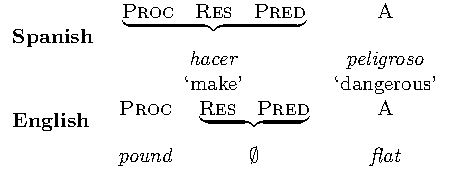
\includegraphics{lexicalization_table}}

\end{document}


